\documentclass[journal]{IEEEtran}
\pagestyle{empty}


\usepackage{cite}

\ifCLASSINFOpdf
  \usepackage[pdftex]{graphicx}
  \graphicspath{{./Images/}}
\else
\fi

\usepackage{algorithmic}

\usepackage{array}
\setlength\extrarowheight{4pt}

\usepackage{caption}
\captionsetup[figure]{font=normal}

\usepackage{url}

\begin{document}

\title{Federation Time}

\author{Manuel Esménio \\ Ponder Source \\ December 2022}% <-this % stops a space

	
\maketitle
\thispagestyle{empty}

\begin{abstract}
	 \cite{Eugene_A._Feinberg-MDP} This paper...
\end{abstract}


\IEEEpeerreviewmaketitle

\section{Background}

\subsection{Federation}

A \textbf{federation} is a group of systems which share data in peer-to-peer transmissions where information flows from a node to its neighbours, while ensuring each individual node maintains \textbf{data sovereignty}, or the ability to choose the access rights of other nodes in federation, thus being able to arbitrarily veto external accesses and modifications  to its own data. 

\begin{figure}[h]
	\hfill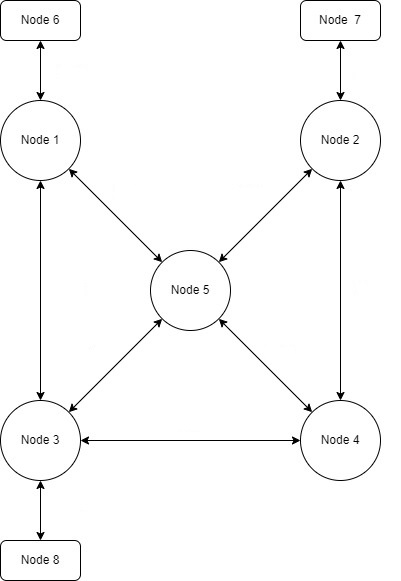
\includegraphics[scale = 0.6]{FEDERATION_1}\hspace*{\fill}
	\caption{Example of a federated system}
	\label{fig:FED1}
\end{figure}

A federation can have both federated and non-federated members. A \textbf {Non-federated member} must have only one neighbour (nodes 6-8 in Fig. \ref{fig:FED1}), and acts as a repository of data (e.g: an API). A \textbf{federated member} must have at least two neighbours (nodes 1-5 in Fig. \ref{fig:FED1}) to forward data as part of a chain of messages without causing duplication issues.

\subsection{Format translation} \label{sect:FORMAT_TRANSLATION}

Part of the problem when building a federated system is the assumption that every node can choose its own syntax. Consider the problem where we want to transfer information between two data repositories, where each uses one of the formats shown in figures \ref{list:FORMAT1} and \ref{list:FORMAT2}, which were copied from the federated timesheets project presented in section \ref{sect:PREV_WORK}:

\begin{figure}[h]

	\begin{itemize}
	
		\item \textbf{Customer} | "Customer1"

		\item \textbf{Project} | "Development"

		\item \textbf{Task} | " "

		\item \textbf{Start time} | "2022-03-30 13:01:00"

		\item \textbf{Stop time} | "2022-03-30 13:25:38"

		\item \textbf{Minutes} | "24"

		\item \textbf{Note} | " "

	\end{itemize}
	\caption{Data fields in format "jiffy-CSV"}
	\label{list:FORMAT1}

\end{figure}

\begin{figure}[h]

	\begin{itemize}
	
		\item \textbf{Date} | "2022-03-30"

		\item \textbf{From} | "14:32"

		\item \textbf{To} | "15:00"

		\item \textbf{Duration} | "1680"

		\item \textbf{Rate} | "KYD 10.00"

		\item \textbf{Internal rate} | "0"

		\item \textbf{User} | "admin"

		\item \textbf{Name} | "admin"

		\item \textbf{Customer} | "Flatley, Purdy and Gerlach"

		\item \textbf{Project} | "Dolore sit"

		\item \textbf{Activity} | "Ea illo"

		\item \textbf{Description} | "test"

		\item \textbf{Exported} | "no"

		\item \textbf{Billable} | "yes"

		\item \textbf{Tags} | "a1,v2"

		\item \textbf{Hourly rate} | "KYD 12.00"

		\item \textbf{Fixed rate} | "KYD 10.00"

		\item \textbf{Type} | "timesheet"

		\item \textbf{label.category} | "work"

		\item \textbf{Account} | "C-37165956"

		\item \textbf{VAT-ID} | "6011598336445140"

		\item \textbf{Order number} | "P-91111562"
	\end{itemize}
	\caption{Data fields in format "kimai-CSV"}
	\label{list:FORMAT2}

\end{figure}

From these formats it is observable that: Some fields can be copy pasted between formats, such as "customer" and "project"; some fields can be reconstructed, for example one can use the "Date" and "From" fields in kimai-CSV and assume the task always starts at 0 seconds to get the "Start time" field from jiffy-CSV, which would probably be acceptable in most use cases in spite of the loss of information; some fields have to be discarded due to one of the formats not containing that information, like the billing information fields which are present in kimai-CSV and not in jiffy-CSV. Since we can't make any assumptions about the language, we can't even be sure \textit{a priori} that the fields "customer" and "project"  are meant to contain the same information, even though they have the same name.

From this example I would like to draw the following conclusions:

\begin{itemize}

	\item In order for two nodes of a federated system to communicate, there must be some logic that handles translating the data being communicated between them.

	\item The loss of information that can potentially arise from the communication between two nodes needs to be expected and accounted for.

	\item Even though an human can design and optimize translation functions, doing so requires some meta-knowledge of the task at hand, such as knowing these formats refer to timesheet tracking apps, which can make the automatization of translation logic for any given pair of nodes a convoluted task.

\end{itemize}

\subsection{Neighbourhood}

In a federated system, the neighbourhood of a node refers to all other nodes it can communicate with (in figure \ref{fig:FED1} the neighbourhood of node 1 is nodes 3,5,6). These communication channels are expected to allow two-way communication and each require their own translation logic, which to summarize what was said in subsection \ref{sect:FORMAT_TRANSLATION} means there is a variable cost to opening each channel.

Consider the problem where we have the federated system schematized in figure \ref{fig:FED1} and we want to transfer data from node 6 to node 7. Using the available communication channels and assuming the message never goes back to a node it has passed through, the possible routes are:

\begin{figure}[h]

	\begin{itemize}
	
		\item $6 \rightarrow 1 \rightarrow 5 \rightarrow 2 \rightarrow 7$

		\item $6 \rightarrow 1 \rightarrow 5 \rightarrow 4 \rightarrow 2 \rightarrow 7$

		\item $6 \rightarrow 1 \rightarrow 5 \rightarrow 3 \rightarrow 4 \rightarrow 2 \rightarrow 7$

		\item $6 \rightarrow 1 \rightarrow 3 \rightarrow 4 \rightarrow 2 \rightarrow 7$

		\item $6 \rightarrow 1 \rightarrow 3 \rightarrow 4 \rightarrow 5 \rightarrow 2 \rightarrow 7$

		\item $6 \rightarrow 1 \rightarrow 3 \rightarrow 5 \rightarrow 4 \rightarrow 2 \rightarrow 7$

	\end{itemize}
	\caption{Routes from node 6 to node 7}
	\label{list:ROUTES1}

\end{figure}

This means that using a strategy where each node forwards the information to all its neighbours, which would be the most resilient for ensuring the information eventually gets to the desired point, requires being able to uniquely identify data transmissions throughout the federation channels, so that the system can prevent the deriving issues of data duplication and infinite message looping.

Altough intuitively the shorter route would be more desirable, there is no guarantee of that, nor that node 5 will not randomly disconnect and require the federation to temporarily operate without it, meaning the neighbourhoods in federated systems have to be carefully designed to prevent geometries that rely on central (and fallible) nodes, while minimizing loss of information and average transmission times across the system.

\subsection{Open/Closed federation}

When one describes the functioning of a federated system one tends to describe a \textbf{open federation}:

\begin{figure}[h]

	\begin{itemize}

		\item Decentralized data transfer system;

		\item Each node has data sovereignty;

		\item Variable and unknown members;

		\item Each node only has information about their neighbours;

		\item No rules, languages or protocols are applied on a global scale;

		\item All issues associated with forwarding data between nodes (duplication, translation, conflicting data, storms) are solved locally by the pairs of neighbours involved;

	\end{itemize}
	\caption{Core ideas of open federation}
	\label{list:FEDOPEN}

\end{figure}

%trust between nodes is a variable that can be used to sort neighbourhoods into optimal configurations.

When one goes to implement a federated system, technological challenges and time restraints often require a solution that does not implement all the requirements in figure \ref{list:FEDOPEN}, or a \textbf{closed federation} system: if there is a fixed and known set of members, we can assume they all trust eachother, which greatly simplifies the problems of transparency and security; if we assume a global rule where data conflicts are solved using "last-write wins" policy, then there is no need for nodes to write their own conflict resolution protocols for all their neighbours, nor their own format translation protocols, which can be hand-crafted  for a known and finite number of members.

The concept of an open federation serve as direction and motivation for the projects currently being developed. While current limitations require our systems to partially operate as a closed federation, the reasoning behind the simplifications used should be explained as part of the implementation details, to set the ground for future work.

\section{Previous work} \label{sect:PREV_WORK}

\section{Current iteration}

\section{Future work}

\section{Glossary}

\subsection{[PLACEHOLDER]}
	In a peer-to-peer data sharing system it feels important to have a quantification of how reliable is the data being transmitted at any given point and time. Such a metric would enable individual nodes to choose between conflicting data (pick the one with highest value), or even to decide whether or not to accept a transmission of data (check if value is above/below a threshold value). 


\bibliographystyle{./IEEEtran}
\bibliography{./Article_Biblio}

	
\end{document}

